\chapter{Experimental part: Models and evaluation / TODO}
\label{chap:model}
In this chapter, we will experiment with the different classification models. We will consider Random Forest, SVM, Extreme Random Forest \cite{ExtRF} and Logistic regression for comparison. Also, we will analyze the feature importance for every event component with Random Forest. We will actively use great Python library scikit-learn.\\

We will do several manipulations before building the model. First of all, we executed missing values imputation with the mean (we replaced outliers with NaN in the previous steps). Then we did standardization with the mean and standard deviation on all numeric features. \\

Also, we implemented custom cross-validation function which tracks the following property: for every train-test split, domains in both sets must not be intersected. The reason for this is following: we have many different URLs, but some of them come from the same domain. Usually, the pages in one domain look similar, and it is not fair to train on some pages and test on the pages from the same domain. Our experimenting showed that if we don't do this, the result of the classifier is overestimated. \\

For every classification model, we add all occurrence of the target event component as positive examples. As negative examples, we add records for random elements from the page and the rest of event components. We use stratification to balance the number of records for both classes.

\section{Feature importance}
To gather the feature importance for every component, we will use Random Forest classifiers. It automatically calculates the "Gini importance" or "mean decrease impurity" which is defined as the total decrease in node impurity, weighted by the probability of reaching that node and then averaged over all trees of the ensemble.\\

Remarkably that the Top-5 features for every component totally makes sense:

\begin{itemize}
    \item \textbf{Event name}: font family, tag, block width, font size, the number of uppercase letters. Usually, the title of the event is bigger and probably has a tag <h1>. The name is rather short, and hence the block width is small. The font size is large and the number of uppercase letters often higher for attracting the user. See figure \ref{fig:importanceName}.
    \item \textbf{Event date}: digits share, the number of digits, font family, tag, number of punctuation. It also logical since the date, of course, has more digits than other web elements. The number of punctuation is rather small because the text is usually short. See figure \ref{fig:importanceDate}.
    \item \textbf{Event location}: number of uppercase letters, tag, font family, the number of siblings, text length.See figure \ref{fig:importanceLocation}.
    \item \textbf{Event description}: block width, text length, font family, number of punctuation. The description, typically, is a wider block of text, that's why block width and text length are the most important features. The number of punctuation is also correlated with the text length and means significant.  See figure \ref{fig:importanceDescription}.
\end{itemize}

\begin{figure}[h]
\begin{center}
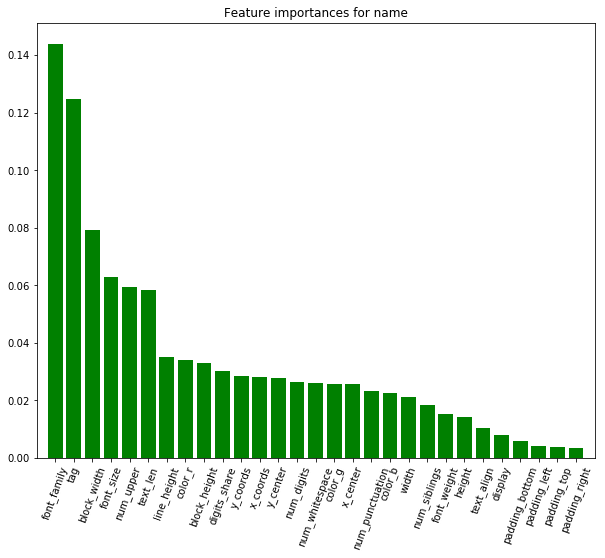
\includegraphics[width=1.0\textwidth]{figures08/importanceName}
\caption{Feature importance from Random Forest for the Event name, Top: font family, tag, block width, font size, number of uppercase letters}
\label{fig:importanceName}
\end{center}
\end{figure}

\section{Comparison of different models}

\subsection{Evaluation metrics}

We used standard metrics for binary classification problem and Information extraction task. All the values reach its best value at 1 and worst score at 0. See below brief description each of them.\\

\noindent\textbf{The mean accuracy} is the average number incorrect predictions 
$$ mean\_accuracy = \frac{tn + fp}{tp + tn + fp + fn}$$
where $tp$, $tn$, $fp$, $fn$ are accordingly true positives, true negatives, false positives and false negatives records from a predicted labels.\\

\noindent\textbf{The precision} is the ability of the classifier not to label as positive a sample that is negative.
$$precision = \frac{tp}{tp + fp}$$ \\

\noindent\textbf{The recall} is the ability of the classifier to find all the positive samples.
$$recall = \frac{tp}{tp + fn}$$ \\

\noindent\textbf{The F1 score}, also known as balanced F-score or F-measure can be interpreted as a weighted average of the precision and recall, where an F1 score. The relative contribution of precision and recall to the F1 score are equal. The formula for the F1 score is:
$$F1 = 2 * \frac{precision * recall}{precision + recall}$$\\

For every pair  (event component, classifier) we will calculate all four metrics, build the summary table and compare the results.

\section{Comparison}

The results of experiments you can see on the talbe \ref{table:sumresult}.
\begin{table}[h]
\begin{center}
{\renewcommand{\arraystretch}{1.2}
\begin{tabular}{lrrrrll}
\toprule
{} &  f1\_score &  accuracy &  precision &  recall &    meta\_name &                  model \\
\midrule
0 &      0.56 &           0.84 &       0.47 &    0.84 &         name &          Random forest \\
0 &      0.00 &           0.89 &       0.18 &    0.00 &         date &          Random forest \\
0 &      0.65 &           0.81 &       0.48 &    1.00 &     location &          Random forest \\
0 &      0.66 &           0.83 &       0.50 &    1.00 &  description &          Random forest \\
0 &      0.61 &           0.82 &       0.44 &    1.00 &         name &                    SVM \\
0 &      0.00 &           0.88 &       0.00 &    0.00 &         date &                    SVM \\
0 &      0.66 &           0.81 &       0.49 &    1.00 &     location &                    SVM \\
0 &      0.66 &           0.83 &       0.50 &    1.00 &  description &                    SVM \\
0 &      0.69 &           0.78 &       0.53 &    1.00 &         name &    Logistic regression \\
0 &      0.00 &           0.85 &       0.12 &    0.00 &         date &    Logistic regression \\
0 &      0.67 &           0.80 &       0.50 &    1.00 &     location &    Logistic regression \\
0 &      0.66 &           0.83 &       0.50 &    1.00 &  description &    Logistic regression \\
0 &      0.51 &           0.87 &       0.57 &    0.67 &         name &  Extreme Random Forest \\
0 &      0.00 &           0.90 &       0.00 &    0.00 &         date &  Extreme Random Forest \\
0 &      0.66 &           0.83 &       0.50 &    1.00 &     location &  Extreme Random Forest \\
0 &      0.66 &           0.83 &       0.50 &    1.00 &  description &  Extreme Random Forest \\
\bottomrule
\end{tabular}}
\caption{Metrics values for a different classification models and event components}
\label{table:sumresult}
\end{center}
\end{table}  \\  